\documentclass{article}
\usepackage{tikz}

\begin{document}

\begin{center}
    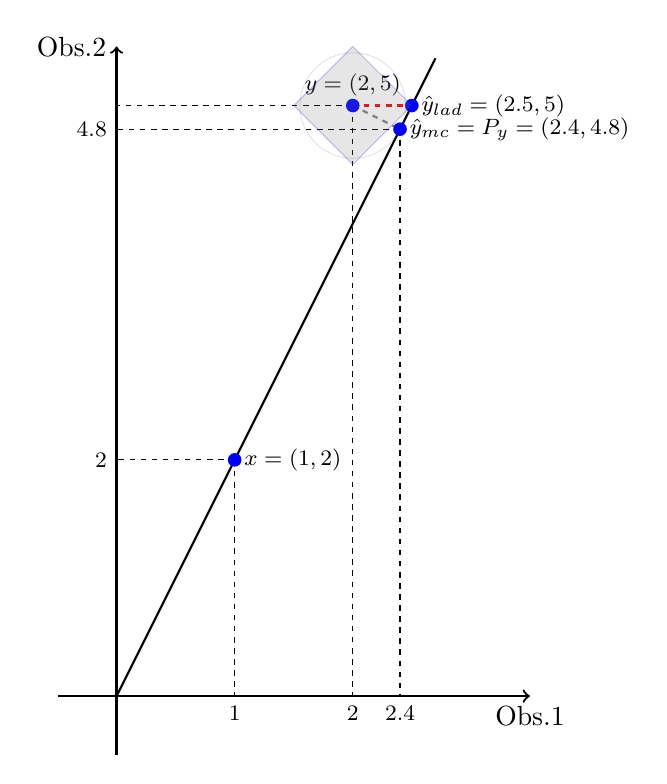
\begin{tikzpicture}[scale=1.5] % Ambos ejes con la misma escala
        
        % Ejes
        \draw[thick,->] (-0.5,0) -- (3.5,0) node[below] {Obs.1}; % Etiqueta eje x
        \draw[thick,->] (0,-0.5) -- (0,5.5) node[left] {Obs.2};  % Etiqueta eje y
        
        % Puntos y líneas auxiliares
        \draw[dashed, dash pattern=on 2pt off 2pt] (1,2) -- (1,0) node[below, font=\footnotesize] {1};
        \draw[dashed, dash pattern=on 2pt off 2pt] (1,2) -- (0,2) node[left, font=\footnotesize] {2};
        
        \draw[dashed, dash pattern=on 2pt off 2pt] (2.4,4.8) -- (2.4,0) node[below, font=\footnotesize] {2.4};
        \draw[dashed, dash pattern=on 2pt off 2pt] (2.4,4.8) -- (0,4.8) node[left, font=\footnotesize] {4.8};
        
        \draw[dashed, dash pattern=on 2pt off 2pt] (2,5) -- (2,0) node[below, font=\footnotesize] {2};
        \draw[dashed, dash pattern=on 2pt off 2pt] (2,5) -- (0,5);
        
        % Recta principal
        \draw[thick] (0,0) -- (2.7,5.4);
             
        % Línea punteada entre Y y P_y (resaltada)
        \draw[thick, gray, dashed, dash pattern=on 2pt off 2pt] (2,5) -- (2.4,4.8);
        \draw[thick, red,  dashed, dash pattern=on 2pt off 2pt] (2,5) -- (2.5,5);
        
        % Círculo centrado en Y y exactamente tangente a la recta en P_y (sin relleno)
        \draw[gray, opacity=0.2] (2,5) circle[radius=0.447];

        % Puntos en azul con etiquetas en negro y tamaño 1.5p
        \filldraw[blue] (1.0,2.0) circle (1.5pt) node[right, text=black, font=\footnotesize] {\footnotesize $x = (1,2)$};
        \filldraw[blue] (2.4,4.8) circle (1.5pt) node[right, text=black, font=\footnotesize] {\footnotesize $\hat{y}_{mc}=P_y=(2.4,4.8)$};
        \filldraw[blue] (2.0,5.0) circle (1.5pt) node[above, text=black, font=\footnotesize] {\footnotesize $y=(2,5)$};
            
        % Agregar el punto (2.5, 5) que es un vértice
        \filldraw[blue] (2.5,5.0) circle (1.5pt) node[right, text=black, font=\footnotesize] {\footnotesize $\hat{y}_{lad}=(2.5,5)$};
        
        % Distancia de Y a Z (0.5)
        \def\dist{0.5} % Distancia entre Y y Z
        
        % Calcular los otros tres vértices del cuadrado
        \coordinate (Y) at (2.0,5.0); % Centro
        \coordinate (Z) at (2.5,5); % Vértice Z

        % Vértice arriba de Y a la misma distancia que Y-Z
        \coordinate (V1) at (2 , 5 - \dist);
        % Vértice abajo de Y a la misma distancia que Y-Z
        \coordinate (V2) at (2 -\dist , 5);
        % Vértice a la izquierda de Z a la misma distancia que Y-Z
        \coordinate (V3) at (2 , 5 + \dist);
        
        % Dibujar el cuadrado con relleno
        \filldraw[blue, fill= gray, opacity=0.2] (Z) -- (V1) -- (V2) -- (V3) -- cycle; % Cuadrado relleno
        
    \end{tikzpicture}
\end{center}

\end{document}





